\textbf{Цель}: "Изучить обучение и функционирование линейной ИНС при решении задач прогнозирования".

\begin{center}
    \textbf{Ход работы}:
\end{center}

\begin{center}
    \textbf{Вариант 5}
\end{center}

\lstinputlisting[
    language=Python,
    name="main.py"
]{../src/main.py}

\newpage

\lstinputlisting[
    name="Консольный вывод",
    basicstyle=\ttfamily\scriptsize
]{input/consoleOut.txt}

График изменения ошибки изображен на рисунке \ref{fig:figure1} (стр. \pageref{fig:figure1}).

\begin{figure}[!htp]
    \center{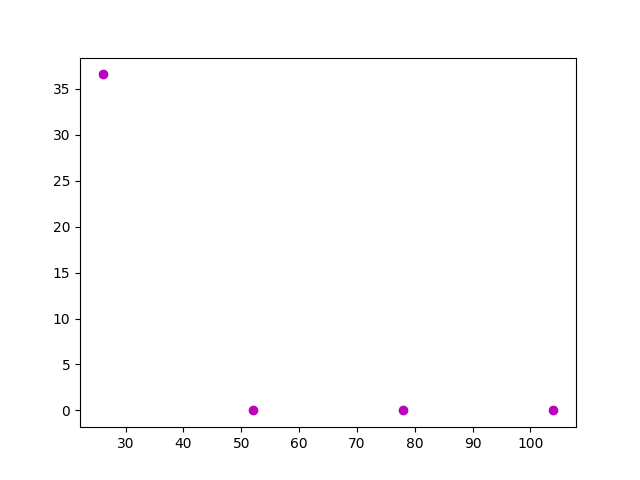
\includegraphics[width=12.5cm]{input/Figure_1.png}}
    \caption{График изменения ошибки}
    \label{fig:figure1}
\end{figure}

\textbf{Вывод}: "Изучили обучение и функционирование линейной ИНС при решении задач прогнозирования".